% Kapitel 6: Infrastruktur, Deployment und Betrieb
\section{Infrastruktur, Deployment und Betrieb}
\label{sec:infrastruktur}

Dieses Kapitel behandelt die infrastrukturellen Komponenten und Prozesse dieser Diplomarbeit.
Erläutert werden unter anderem der Deployment-Prozess sowie die im laufenden Betrieb relevanten Aspekte wie Monitoring und Logging, Datenbank-Management und Backup-Strategien.


\subsection{Container-Orchestrierung}
\label{sec:container_orchestrierung}

Die gesamte Applikation wird mittels Docker Compose orchestriert, wobei zwei separate Konfigurationsdateien für die Entwicklungs- und Produktionsumgebungen benutzt werden.
Docker Compose nutzt, wie bereits im entsprechenden Kapitel erwähnt, YAML-Dateien, welche zur Unterscheidung mit den Endungen \texttt{.prod.yaml} und \texttt{.dev.yaml} versehen wurden.
Beide Konfigurationen definieren dieselben Services, unterscheiden sich jedoch grundlegend in der Art und Weise, wie diese für Docker zum Starten bereitgestellt werden.


\subsubsection{Entwicklungsumgebung}

In der Entwicklungsumgebung werden alle Services lokal aus ihren jeweiligen Dockerfiles gebaut.
Ein zentrales Merkmal ist die Verwendung von Volume-Mounts, welche lokale Dateiverzeichnisse direkt in die Container einbinden:

\begin{lstlisting}[language=yaml, caption={Volume Mount Entwicklungs-Compose-Konfiguration}, label={lst:compose_dev}]
data-collection-service:
  build:
    context: ./services/data-collection-service
    dockerfile: Dockerfile
  volumes:
    - ./services/data-collection-service/src:/app/src:rw
\end{lstlisting}

Durch diese Konfiguration werden Codeänderungen sofort im laufenden Container wirksam (Hot-Reload), ohne dass der Container neu gebaut werden muss.
Dies beschleunigt den Entwicklungszyklus erheblich, da Änderungen am Quellcode schnell in der Docker-Umgebung getestet werden können.

\newpage
\subsubsection{Produktionsumgebung}

Die Produktionskonfiguration verwendet hingegen vorgefertigte Docker-Images, welche über eine Docker-Registry heruntergeladen werden:

\begin{lstlisting}[language=yaml, caption={Image Produktions-Compose-Konfiguration}, label={lst:compose_prod}]
data-collection-service:
  image: julianbierbaum/license-plate-system:data-collection-service
  restart: unless-stopped
\end{lstlisting}

Die Volume-Mounts für den Quellcode entfallen hier vollständig, da dieser direkt in die zuvor gebauten Images eingebettet wurde.
Eine wichtige Ausnahme hierbei ist allerdings das Volume der Datenbank, welches für den Bestand der Daten weiterhin außerhalb des Images gespeichert wird.
Dies bedeutet, dass diese Images eigenständig sind und alle Abhängigkeiten sowie den Applikationscode bereits enthalten.

Für das Deployment auf der Produktionsumgebung werden daher ausschließlich die Docker Compose-Datei und die Umgebungsvariablen zur Konfiguration benötigt, ein Klonen des Quellcode-Repositories ist nicht erforderlich.
Dies ist für die Nutzung von Portainer wichtig, ein Tool, welches später in diesem Kapitel näher beleuchtet wird.
Zusätzlich wurde die Restart-Policy strikter gesetzt, um sicherzustellen, dass Container nach einem Absturz oder einem Neustart des Host-Systems automatisch wieder hochgefahren werden.


\subsubsection{Startabhängigkeiten und Healthchecks}

Ein wesentlicher Aspekt der Orchestrierung ist die korrekte Startreihenfolge der Services.
Da alle Applikationsservices eine funktionierende Datenbank voraussetzen, wird ein spezieller Datenbank-Prestart-Container eingesetzt, welcher die Datenbank initial konfiguriert.
Erst wenn dieser Container erfolgreich durchgelaufen ist, werden die abhängigen Services gestartet:

\begin{lstlisting}[language=yaml, caption={Startabhängigkeiten Datenbank Prestart}, label={lst:compose_depends}]
depends_on:
  db-prestart:
    condition: service_completed_successfully
\end{lstlisting}

Der Prestart-Service wartet selbst wiederum auf den PostgreSQL-Container, welcher über einen Healthcheck seine Bereitschaft signalisiert.
Zusätzlich verfügen die Backend-Services und der Plate Recognizer-Container über eigene Healthchecks, mit welchen, über definierte HTTP-Endpunkte der aktuellen Zustand eines Services überwacht werden kann.

\newpage
\subsection{CI/CD Pipelines und Deployment}
\label{sec:cicd}

CI/CD (Continuous Integration / Continuous Delivery) bezeichnet die Praxis, Codeänderungen automatisiert zu testen, bauen und bereitzustellen \cite{redhat_cicd}.
Continuous Integration stellt sicher, dass Codeänderungen automatisch auf Fehler geprüft werden, bevor diese in den Hauptbranch des Code-Repositories aufgenommen werden.
Continuous Delivery automatisiert darauf aufbauend den Build- und Bereitstellungsprozess, sodass neue Versionen automatisch in der Docker-Registry als Images zur Verfügung gestellt werden.

Die Umsetzung dieser Prinzipien erfolgt im Projekt über GitHub Actions, ein in GitHub integriertes Automatisierungstool, mit welchem Workflows zum Bauen, Testen und Bereitstellen von Software direkt im Repository definiert werden können.
Diese Prozesse werden durch Ereignisse wie Code-Pushes oder Merges automatisch ausgelöst und führen die konfigurierten Schritte auf virtuellen Servern aus. \cite{github_actions}

\subsubsection{Build und Test Pipeline}

Die primäre CI/CD-Pipeline wird bei jedem Push auf einen beliebigen Branch ausgelöst und besteht aus zwei sequenziellen Phasen:

\paragraph{Phase 1: Testing und Linting}
In der ersten Phase werden für jeden Python-Service automatisiert drei Prüfungen durchgeführt:

\begin{enumerate}
  \item Formatierung (Ruff Format \cite{ruff_formatter}): Überprüfung des Codes auf Einhaltung der definierten Formatierungsregeln.
  \item Linting (Ruff Check \cite{ruff_linter}): Statische Codeanalyse zur Erkennung von potenziellen Fehlern und Stilabweichungen.
  \item Tests (Pytest mit Coverage): Ausführung aller Test-Cases, welche mit einer Codeabdeckungsanalyse kombiniert werden.
\end{enumerate}

Alle Tests werden innerhalb von Docker-Containern ausgeführt, um eine konsistente und reproduzierbare Testumgebung zu gewährleisten, welche der Produktionsumgebung möglichst nahekommt.

\newpage
\paragraph{Phase 2: Build und Push}
Wenn die Testphase erfolgreich abgeschlossen wurde und der Push auf dem Haupt-Branch erfolgt, wird die zweite Phase ausgelöst.
Diese nutzt ein Build-Script, welches automatisiert alle Docker-Images baut und in die definierte Registry pusht.

\begin{lstlisting}[language=bash, caption={Auszug Build-Script \texttt{build.sh}}, label={lst:build_script}]
# Build all services
for SERVICE_DIR in services/*/; do
  SERVICE_NAME=$(basename "$SERVICE_DIR")
  echo "--- Building ${SERVICE_NAME} ---"

  # Check Python lock file
  if [ -f "${SERVICE_DIR}pyproject.toml" ] && [ ! -f "${SERVICE_DIR}uv.lock" ]; then
    echo "Error: ${SERVICE_DIR}uv.lock not found. Run uv sync first."
    exit 1
  fi

  # Check Node.js lock file
  if [ -f "${SERVICE_DIR}package.json" ] && [ ! -f "${SERVICE_DIR}package-lock.json" ]; then
    echo "Error: ${SERVICE_DIR}package-lock.json not found. Run npm install first."
    exit 1
  fi

  docker build -t "${DOCKER_REGISTRY}:${SERVICE_NAME}" "$SERVICE_DIR"
  docker push "${DOCKER_REGISTRY}:${SERVICE_NAME}"
done
\end{lstlisting}

Dieses iteriert, wie im Code-Ausschnitt zu sehen ist, über alle Service-Verzeichnisse und identifiziert dabei Services anhand ihrer Lock-Files.
Da für die Python-Services UV als Package Manager benutzt wurde, dient das \texttt{uv.lock}-File als Identifikationsmerkmal für diese.
Frontend-Services werden mittels des \texttt{package-lock.json}-Files identifiziert und alle anderen Services, welche nicht im Service-Verzeichnis liegen, werden separat aufgerufen.
Das vollständige \texttt{build.sh}-Script ist im Anhang einsehbar.

\newpage
\subsubsection{Deployment mit Portainer}

Deployment auf der Produktionsumgebung erfolgt über die Plattform Portainer, ein Container Management-Tool mit Weboberfläche \cite{portainer}.
Portainer wurde auf dem Synology-NAS installiert und ermöglicht das Verwalten der Docker-Container direkt über einen Browser.

Für das Deployment wird in Portainer ein Stack erstellt, welcher die Produktions-Compose-Datei sowie die Datei mit den Umgebungsvariablen enthält.
Bei Aktualisierungen werden die neuesten Images aus dem Docker-Registry heruntergeladen, woraufhin die betroffenen Container automatisch neu erstellt werden, ohne dass die Datenhaltung betroffen ist.

\begin{figure}[htbp]
  \centering
  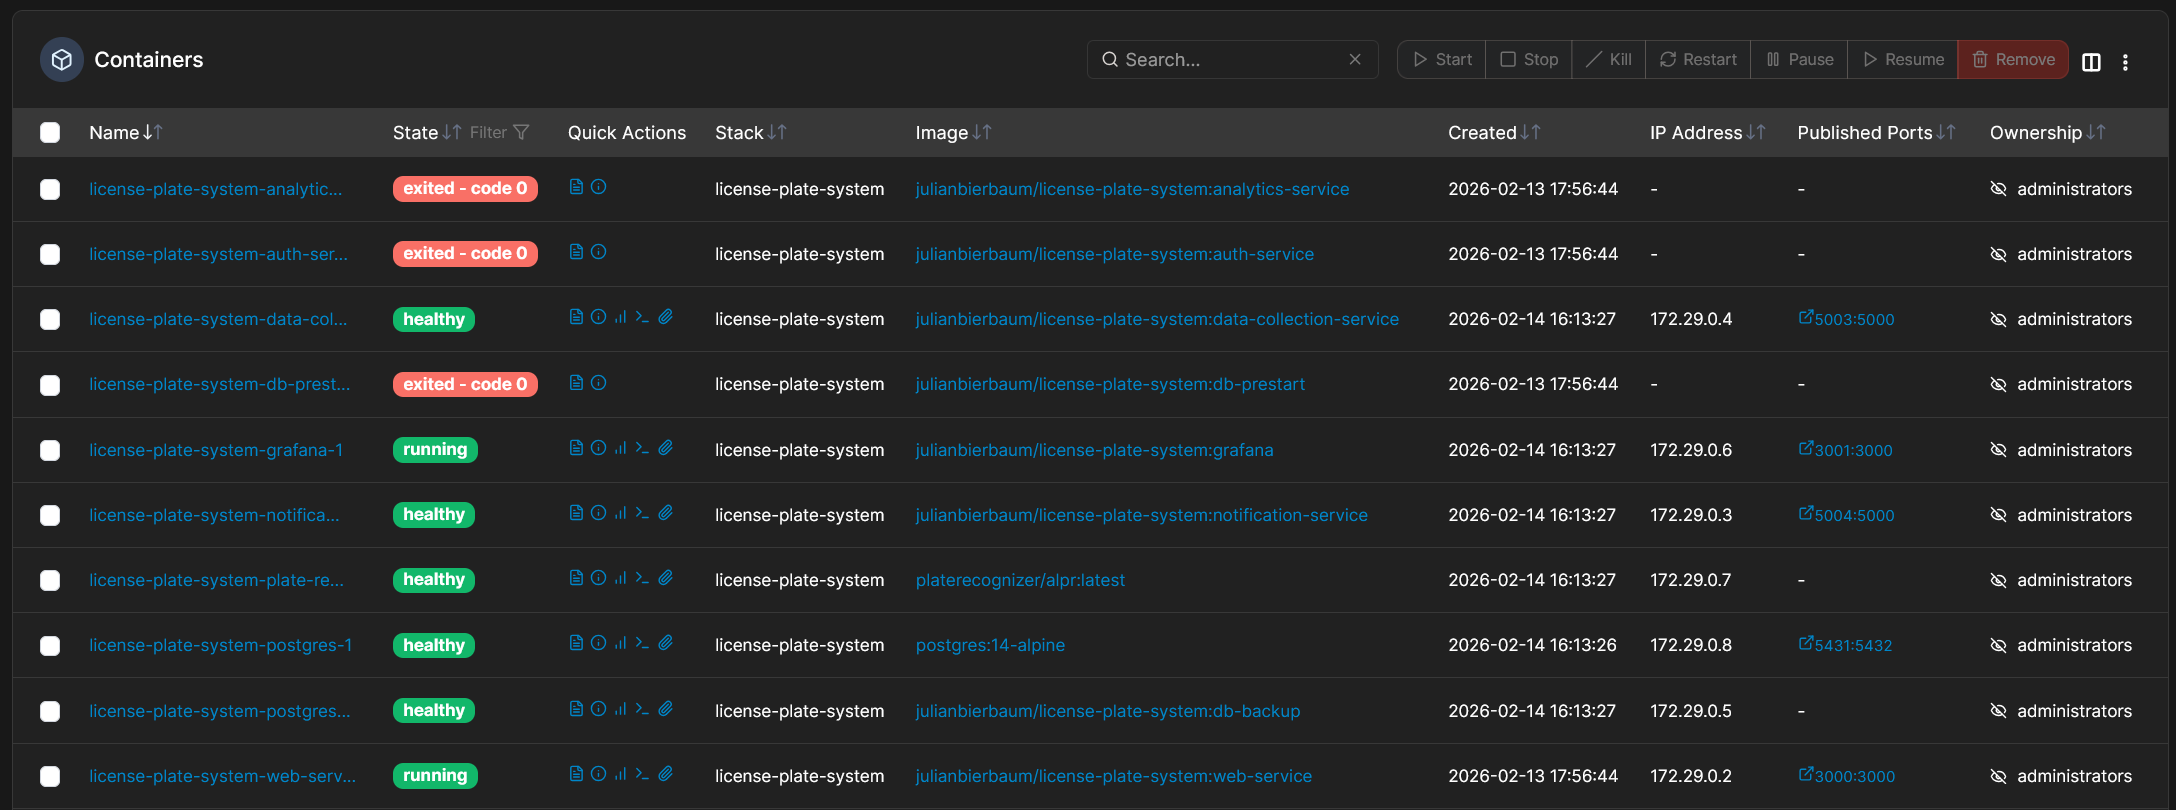
\includegraphics[width=\textwidth]{container_stack_portainer.png}
  \caption{Laufender Container-Stack in Portainer}
  \label{fig:portainer}
\end{figure}

\newpage
\subsection{Monitoring und Logging}


\subsubsection{Healthchecks}

Wie bereits erwähnt (Kapitel~\ref{sec:container_orchestrierung}) verfügen die Services über Healthchecks, welche von Docker Compose in regelmäßigen Intervallen (alle 5 Sekunden) ausgeführt werden und primär dazu dienen, die Verfügbarkeit der Services zu überwachen.
Die Methode des Healthchecks variiert je nach Service-Art:

\begin{itemize}
  \item Backend-Services (Data Collection, Notification): HTTP-Request an den \texttt{/health}-Endpunkt des jeweiligen Services.
  \item PostgreSQL-Datenbank: Verwendung des nativen \texttt{pg\_isready}-Kommandos zur Überprüfung der Datenbankbereitschaft.
  \item Plate Recognizer: HTTP-Request an den Root-Endpunkt des ALPR-Containers.
  \item Backup-Service: Überprüfung, ob der Cron-Daemon (\texttt{crond}) als Prozess läuft.
\end{itemize}

Der Status der Healthchecks ist über Portainer einsehbar und ermöglicht somit eine zentrale Überwachung des Status aller Container.


\subsubsection{Logging}

Alle Services wurden so konfiguriert, dass Log-Ausgaben direkt auf die Konsole geschrieben werden (Console-Logging).
Das Log-Level ist über eine Umgebungsvariable konfigurierbar und wird in der Produktionsumgebung typischerweise auf INFO gesetzt, während in der Entwicklungsumgebung DEBUG als Standard dient.

Die Logs sind über Docker und Portainer einsehbar.
Durch die Verwendung des Python Logging-Moduls in allen Backend-Services wird ein einheitliches Log-Format erzeugt, welches Zeitstempel, Log-Level und den Namen des Services enthält, auf welchem der Log erstellt wurde.

\begin{lstlisting}[caption={Beispielhafte Log-Ausgabe des Data Collection Services}, label={lst:log_example}]
2026-02-17 15:55:24,782 - data-collection-service - INFO - Vehicle detected from camera: BC500-001
2026-02-17 15:55:26,461 - data-collection-service - INFO - No vehicle observations found in reader result.
\end{lstlisting}

Des Weiteren könnte dieses Modul zukünftig erweitert werden, um etwa gleichzeitig mit dem Console-Log in zentrale Log-Files zu schreiben.

\newpage
\subsection{Datenbank-Management}


\subsubsection{Initiale Einrichtung}

Die initiale Einrichtung der Datenbank erfolgt automatisch beim ersten Start des Systems über den DB-Prestart-Container.
Dieser führt ein Entrypoint-Script aus, das zwei Aufgaben erfüllt:
Zunächst führt dieser ein Init-Script aus. Dieses SQL-Script erstellt die spezifischen Datenbank-Schemas und -Benutzer der Services, welche bereits im Kapitel~\ref{sec:db_architektur} erläutert wurden.
Zudem werden die granularen Berechtigungen vergeben, wie sie im Sicherheitskonzept (Abschnitt~\ref{sec:db_zugriff}) definiert wurden, beispielsweise erhält der Analytics-Service-User nur Leserechte auf das Ingestion-Schema.

Die zweite Aufgabe dieses Services ist die Ausführung der Datenbankmigrationen unter Benutzung von Alembic.
Nach der zuvor erwähnten Schema-Erstellung werden automatisch alle ausstehenden Migrationen angewendet, um die Tabellen in den aktuellen Zustand zu bringen.
Durch diese automatisierte Einrichtung entfällt jegliche manuelle Datenbankadministration beim initialen Deployment oder beim Neuaufsetzen des Systems.

Das init.sql-Script ist im Anhang angeführt.


\subsubsection{Schema-Migrationen mit Alembic}

Für die Versionierung des Datenbankschemas wird Alembic eingesetzt, ein Migrationswerkzeug für SQLAlchemy-basierte Anwendungen.

Der DB-Prestart-Container kopiert die SQLAlchemy-Modelle der einzelnen Services in den eigenen Build-Kontext und kann somit das Schema aller Services zentral verwalten. \cite{alembic_monorepo}
Diese sind mittels Volumes aus den Verzeichnissen der Backend-Services an den Prestart-Container angebunden.

\begin{lstlisting}[language=bash, caption={Dockerfile COPY Anweisungen}, label={lst:prestart_copy}]
COPY services/data-collection-service/src/ /app/data_collection/src/
COPY services/notification-service/src/ /app/notification/src/
# COPY services/analytics-service/src/ /app/analytics/src/
\end{lstlisting}

\newpage
Die Alembic-Konfiguration importiert die Base-Klassen der Backend-Services im Environment-Python-File:

\begin{lstlisting}[language=python, caption={Alembic target\_metadata}, label={lst:alembic_env}]
# Import Base objects
from data_collection.src.models.base import IngestionBase
from notification.src.models.base import NotificationBase
# from analytics.src.models.base import AnalyticsBase

target_metadata = [
    IngestionBase.metadata,
    NotificationBase.metadata,
    # AnalyticsBase.metadata,
]
\end{lstlisting}

Durch diesen zentralisierten Ansatz können Migrationen generiert werden, welche über alle Schemas hinweg konsistent sind.
Die Migrationen werden wie bei Alembic üblich versioniert und mit dem Repository eingecheckt, wobei jede Migration durch eine Python-Datei repräsentiert wird, welche sowohl die Up- als auch Downgrade-Funktion enthält, um Schema-Änderungen vorwärts und rückwärts anwenden zu können.

\newpage
\subsection{Backup-Strategie}

Die Backup-Strategie des Systems umfasst sowohl automatisierte als auch manuelle Sicherungsmechanismen und einen manuellen Wiederherstellungsprozess.


\subsubsection{Automatisiertes Backup}

Für die automatisierte Sicherung der PostgreSQL-Datenbank wird ein dedizierter Backup-Container eingesetzt, welcher als separater Service im Docker Compose-Stack definiert wurde.
Dieser Container basiert auf dem offiziellen PostgreSQL-Alpine-Image und nutzt den Cron-Daemon zur zeitgesteuerten Ausführung des Backup-Scripts.

Der Backup-Zeitplan wird über die Umgebungsvariable \texttt{BACKUP\_SCHEDULE} im Cron-Format konfiguriert (In diesem Fall etwa \texttt{0 2 * * *} für ein tägliches Backup um 02:00 Uhr \cite{cron_guru}).
Falls die Variable nicht gesetzt wurde, werden automatische Backups deaktiviert und der Container wechselt in einen Idle-Zustand.

\begin{figure}[htbp]
  \centering
  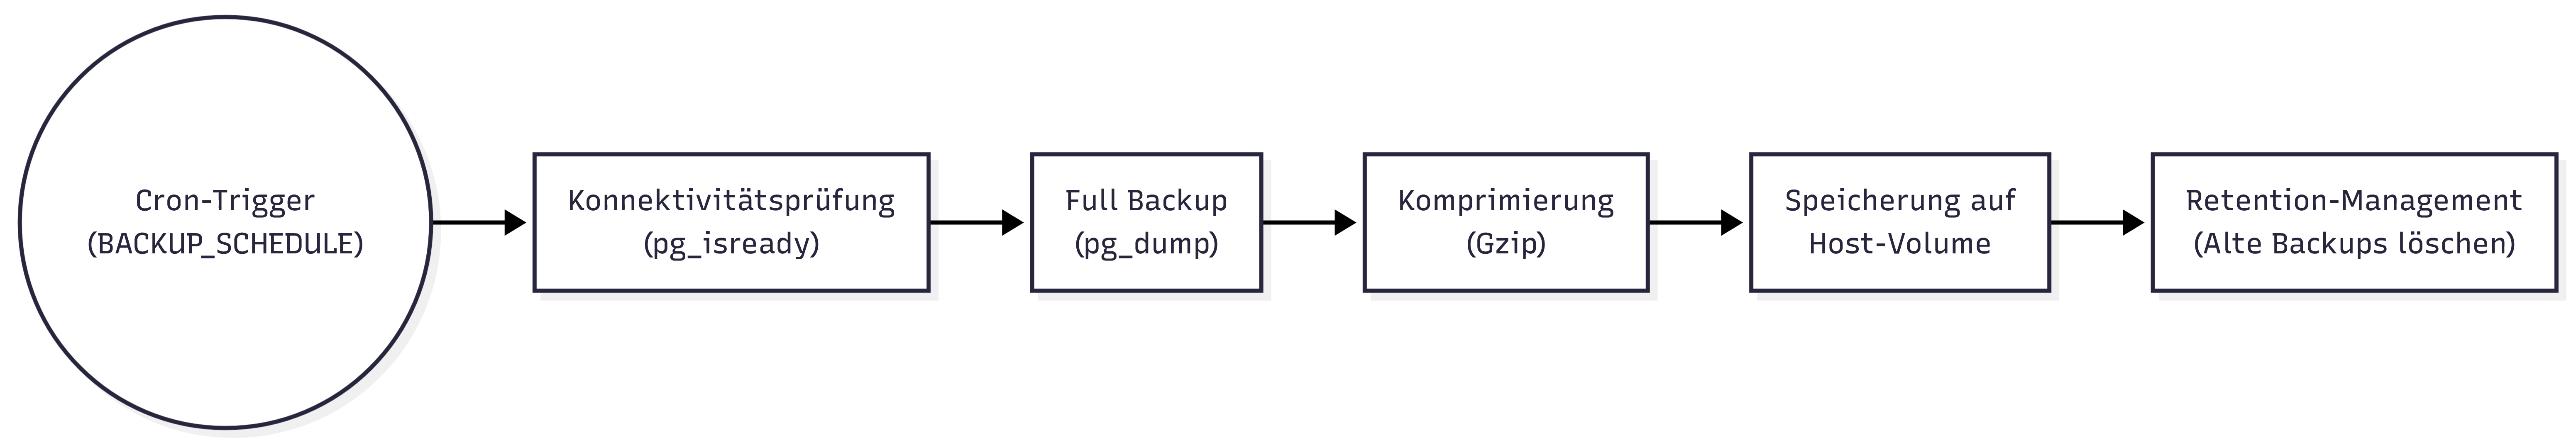
\includegraphics[width=\textwidth]{backup_flow.png}
  \caption{Backup Flow}
  \label{fig:backup_flow}
\end{figure}

Der Cron-Daemon löst das Backup-Script zum konfigurierten Zeitpunkt aus.
Dieses wartet zunächst auf die Erreichbarkeit der Datenbank, erstellt dann einen vollständigen Datenbank-Dump mittels \texttt{pg\_dump} \cite{postgres_pgdump}, komprimiert anschließend diesen mit Gzip und schreibt die entstandene Backup-Datei auf ein gemountetes Host-Volume.
Abschließend werden Backups, die älter als die konfigurierte Aufbewahrungsdauer (standardmäßig 30 Tage) sind, automatisch gelöscht.

In dieser Implementierung wird bei jedem Durchlauf ein vollständiges Datenbank-Backup (Full Backup) erstellt, anstatt auf inkrementelle oder differentielle Strategien zurückzugreifen.
Wie im Kapitel zur Datenbankarchitektur (\ref{sec:denormalisierung}) errechnet, beträgt die Größe eines komprimierten Full-Backups selbst bei über 60.000 gespeicherten Erkennungen lediglich rund 3,4 MB.
Bei diesen Größenordnungen bringt eine inkrementelle Strategie keinen nennenswerten Vorteil, würde jedoch die Komplexität der Wiederherstellung erhöhen, da inkrementelle Backups stets auf einem vollständigen Basis-Backup aufbauen und in korrekter Reihenfolge eingespielt werden müssen.


\subsubsection{Manuelles Backup und Wiederherstellung}

Zusätzlich zu den automatisierten Backups steht ein manuelles Backup-Script zur Verfügung.
Dieses startet einen temporären PostgreSQL-Container, der den Dump erstellt und anschließend sofort wieder entfernt wird.
Ansonsten ist dieser funktionell gleich aufgebaut, wie das oben aufgezeigte System für automatisierte Backups.

Für die Wiederherstellung existiert ebenfalls ein Script, welches einen vollständigen Disaster-Recovery-Prozess implementiert:

\begin{figure}[htbp]
  \centering
  
\includegraphics[width=1.1\textwidth]{restore_flow.png}
  \caption{Restore Flow}
  \label{fig:restore_flow}
\end{figure}

Das Script fordert zunächst eine explizite Bestätigung, da alle in der Datenbank bestehenden Daten überschrieben werden müssen.
Anschließend werden alle aktiven Datenbankverbindungen terminiert, die bestehende Datenbank gelöscht und neu angelegt, bevor das komprimierte Backup mittels \texttt{pg\_restore} \cite{postgres_pgrestore} eingespielt wird.

Das Recovery Point Objective (RPO) entspricht dem konfigurierten Backup-Intervall (standardmäßig 24 Stunden), das Recovery Time Objective (RTO) beträgt einige Sekunden bis wenige Minuten und ist primär durch die Größe des Backups bestimmt.

\subsection{Documentation as Code (MkDocs)}

Die Entwicklerdokumentation wird im Repository gepflegt und automatisiert, mithilfe von GitHub Pages \cite{github_pages}, veröffentlicht.
Hierfür wird MkDocs \cite{mkdocs} mit dem Material-Theme \cite{mkdocs_material} eingesetzt, ein Python-basierter Static-Site-Generator, welcher Markdown-Dateien in eine Dokumentationswebsite transformiert.
Die Verwendung von MkDocs hat den Vorteil, dass out-of-the-box viele Grundfunktionen einer guten Dokumentation, wie etwa eine Navigationsleiste oder Suchfunktion, bereits als Module funktionsfähig bereitgestellt werden.

Die Dokumentation ist in sechs Hauptbereiche gegliedert:
\begin{itemize}
  \item Getting Started Voraussetzungen, Installation und Konfiguration für neue Entwickler
  \item Development: Entwicklungsumgebung, Docker-Befehle und Service-Entwicklung
  \item Operations: Backup-Verfahren, Wiederherstellung und Monitoring
  \item Deployment: Übersicht, Image-Erstellung und Produktionseinrichtung
  \item Reference: Script-Referenzen, Docker-Compose-Dokumentation, API-Dokumentation und Data-Collection-Flow
\end{itemize}

Die Veröffentlichung von Änderungen erfolgt automatisiert über einen eigenen GitHub-Actions-Workflow.
Im Falle eines Pushes wird die Dokumentation neu gebaut und auf GitHub Pages veröffentlicht.
Dadurch ist die Dokumentation stets synchron mit dem aktuellen Stand des Codes und unter einer permanenten, öffentlichen URL erreichbar.

Dieser Ansatz folgt dem Documentation-as-Code-Prinzip, bedeutet, dass die Dokumentation derselben Versionskontrolle wie der Quellcode unterliegt und Änderungen denselben Review-Prozess (Pull Requests) durchlaufen.
Dies hat in der Entwicklung den großen Vorteil, dass die Dokumentation als Teil der Code-Basis gesehen und verwaltet wird und so einfacher und schneller bei Änderungen angepasst werden kann.

\begin{figure}[htbp]
  \centering
  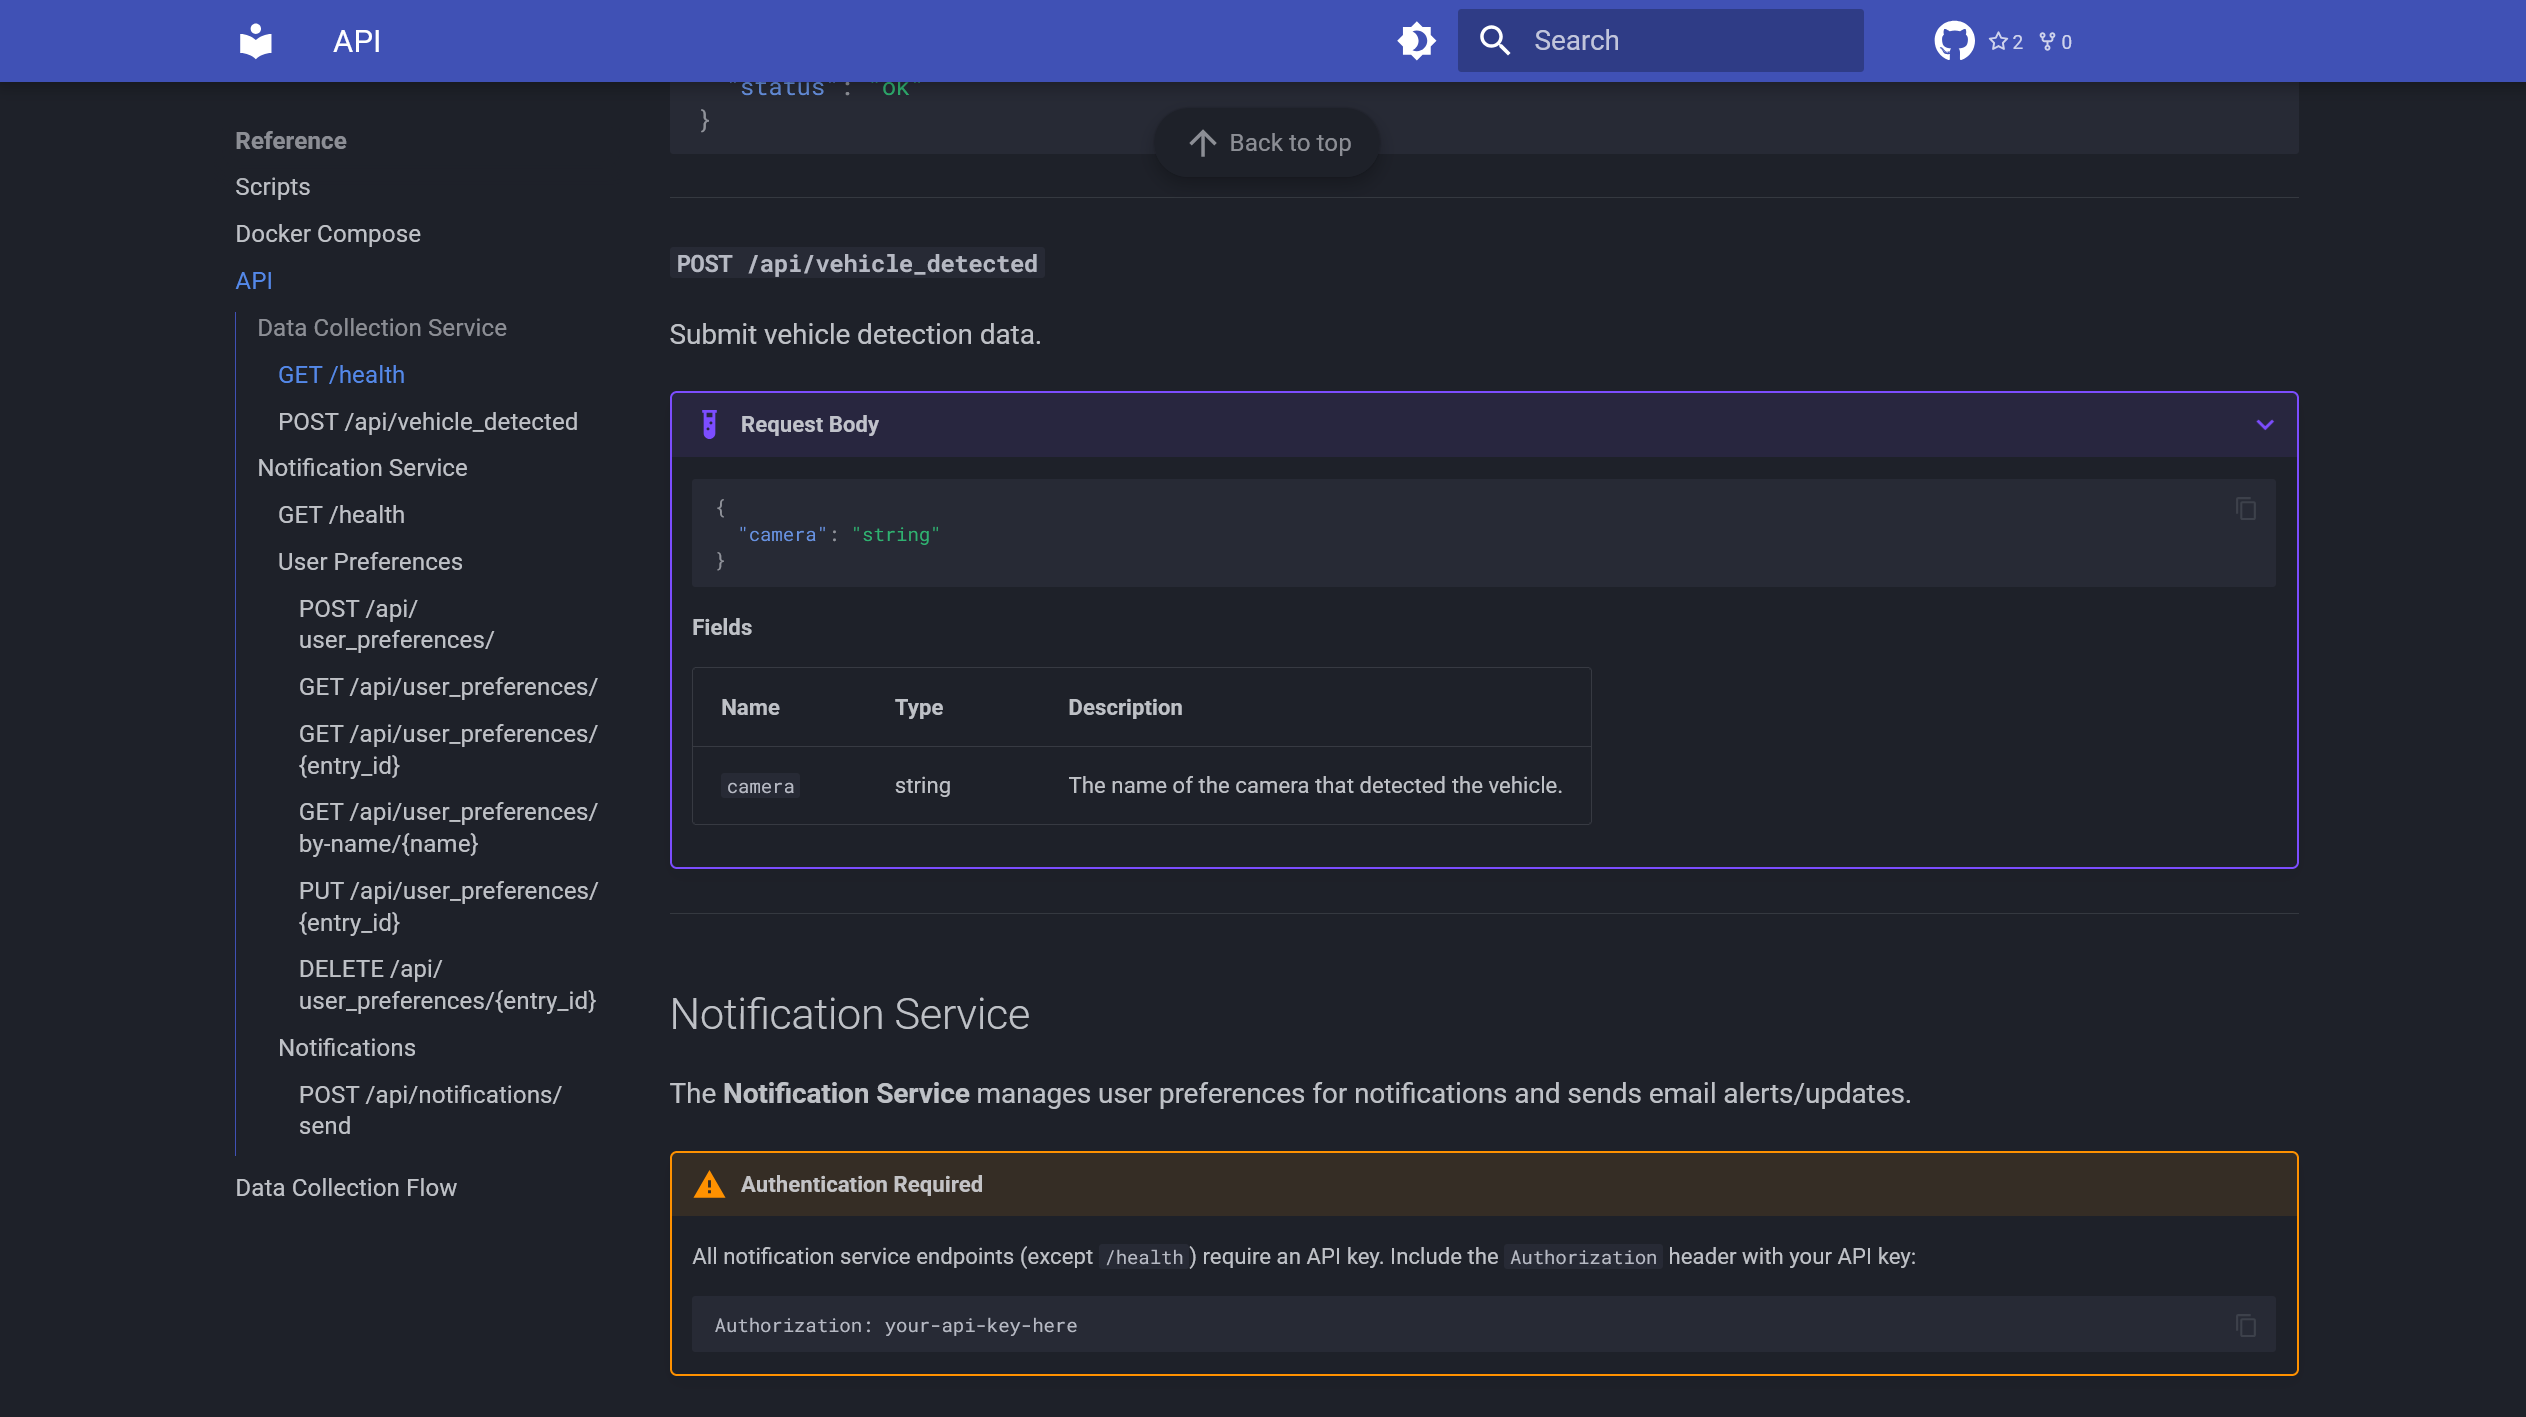
\includegraphics[width=\textwidth]{mkdocs.png}
  \caption{Entwicklerdokumentation mittels MkDocs}
  \label{fig:mkdocs}
\end{figure}
